\iffalse
\section{writeup from 2022/01/21}
The disagreements on anatomical classification implies the need to a metric of confidence on the detection and characterization of brain structures.
The difficulty or ease of detecting a structure is variable. 
In any particular brain, some structures are detected consistently by anatomists while others are not.
The challenge in making the system usable to the anatomists is first to automatically detect structures and second, to provide an explanation for its detections and an associated confidence.

Our goal in the design of the system is to create models of the brain
that can be explained to, and modified by, anatomists. In other words,
we take a white box, rather than a black box approach.

This impacts the design in several important ways. First, image
analysis methods in general, and CNNs in particular, are based on
concept of a sliding window. In other words, the basic unit of
analysis is a rectangular area, whose location is indpendent of the
content of the image. In contrast our analysis unit is the image of a
single cell.~\footnote{When cells are overlapping we sometimes get
  the image of several scells as the unit.} By annotating cells we
visually explain to the anatomist the basis for the computer's
decision.

Second, we represent each cell by a set of features. the basic 
features are size, aspect ratio, and orientation. To characterize the
cell shape beyond these basic features, we use an unsupervised
learning method to find a dimensionality reducing mapping from cell
image to ten additional parameters. We demonstrate that this
unsupervised method provides a consistent parameterization across
brains and across imaging modalities.

Third, explaining structure detection (xxxx).



\section{Adaptive parametrization of cell shapes}
\label{sec:DM}
In this section we describe the two main technical contributions of this
paper: a method for learning a cell-shape feature-set that is optimized
for a particular brain, and a method for mapping between feature-sets
from different brains. Both methods are {\em unsupervised}, in other
words, the input to these methods are sets of sections with no
annotation or alignment.

The first step is to segment individual cells from the section
image. For this we use a locally adaptive variant of
Otsu's method~\cite{otsu1979threshold}. This step is not perfect, over and under segmentations are
common. However, our method relies on the statistical properties for
many cells, which greatly reduces the sensitivity of the analysis to
segmentation errors. 
Cell patches are typically $50\times 50$ pixels which is a highly
redundant representation. The second step is to
map the cell image to a less redundant low-dimensional representation. Our goal here
is to find a small set of features (10) that represent shapes of cells
from a given brain. Our learned features provide a better representation 
of cells shapes which contrast with the feature extraction stage in~\cite{chen2019active}, 
which uses a pre-trained CNN (Inception-BN). 


We use Diffusion Maps
(DM)~\cite{belkin2003,coifman2005geometric}~\footnote{{\tt
    https://github.com/DiffusionMapsAcademics/pyDiffMap}} to find a
low dimensional representation of cell shapes. While DM has gained
popularity in many applications, the only work we are aware of
regarding the use of DM for cell shape analysis is in the context of
differentiation lineages~\cite{haghverdi2015diffusion}.
The public implementation of DM is excellent. However, it is limited to datasets that
fit in computer memory. As we typically extract from each brain
hundreds of millions of cells, we need an efficient way to create a
small number of representative patches.  We use a streaming version of
the Kmeans++~\cite{arthur2006k} seeding algorithm followed with a few
iterations of Kmeans. Figure~\ref{fig:kmeans} shows samples of the
original cell images and of cells after normalizing
rotation, Kmeans++ and Kmeans averaging.
\begin{figure}[t]
  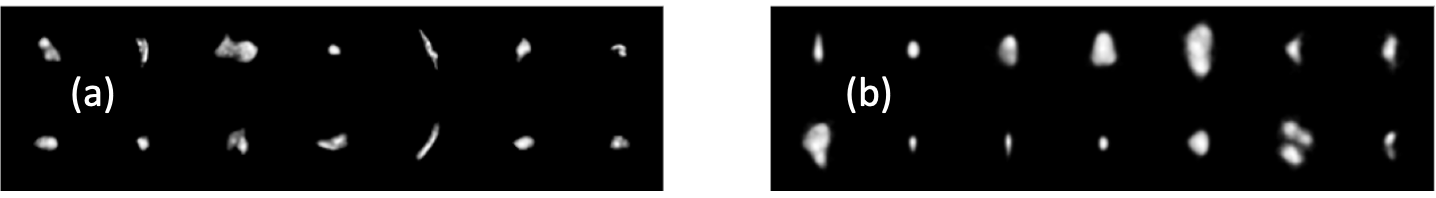
\includegraphics[width=\textwidth]{Images/CellImages.png}
\caption{{\bf (a)} a sample of Cell patches,
  {\bf (b)}  a sample of the orientation-normalized, Kmeans-reduced and averaged cell images.}
\label{fig:kmeans}
\end{figure}

DM~\cite{coifman2005geometric} creates a continuous
non-linear mapping from single cell patches into a ten component
feature vector. The ten components correspond to ten most dominant
(lowest non-zero eigenvalue) eigen-vectors of the Laplace-Beltrami
operator. We conceptualize the DM of a population of cells as
a ten dimensional cloud of patches, each patch placed at the location
defined by the corresponding feature vector. By projecting this cloud
onto a two dimensional plane, we generate a visualization of the patch
cloud (see figure~\ref{fig:diffusionmap}).

After inspecting patch clouds from several brains, it became clear
that the clouds corresponding to different brains are similar. More
precisely, the clouds all have similar shapes when projected on
different planes, but the order of and orientation can be
different. This gave us the idea that there might be a single {\em
  universal} set of features, such that one can map the shape-features from
any brain to this universal set of features.

Such a universal set of features provides several benefits. First, it
provides a way to visualize the difference between regions in terms of
the density, types and orientations of cells. This gives
the anatomist a way to understand the decisions made by the computer
and potentially correct them. This is in contrast with black box
methods such as deep neural networks which provide no explanations of
their decisions.

\begin{figure} [t]
  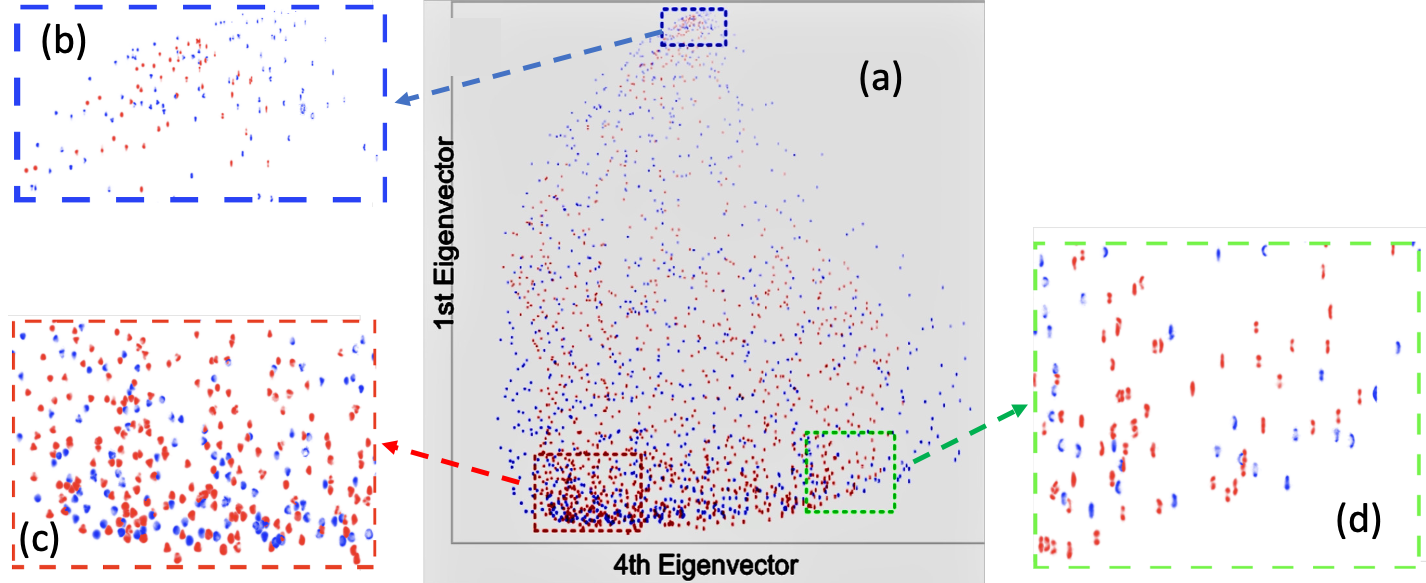
\includegraphics[width=\textwidth]{Images/Scatter.png}
\label{fig:diffusionmap}
\caption{{\bf Projecting the patch cloud and universal features}. This
  figure demonstrates the continuous mapping generated by DM. {\bf
    (a)} shows the projection of two patch clouds on the first and
  fourth eigenvectors produced by DM. The red patches correspond to
  cells stained by Thionin and imaged using brightfield, the blue
  patches correspond to cells stained with Neurotrace blue and imaged
  using fluorescent imaging. The brightfield cloud has been
  transformed to match the fluorescent cloud. Observe that the shape
  of the clouds match closely. Further, the insets show that the cell
  shapes match as well.  {\bf (b)} corresponds to very
  small cells. {\bf (c)} correspond to large and round cells, and {\bf
    (d)} correspond to thin cells or a row  of 2-3 cells.}
\end{figure}
Second, using a universal set of features decouples any downstream processing from
variations in section preparation and imaging. Such decoupling is particularly
valuable when switching between different imaging modalities such as
fluorescence vs. brightfield. In the next section we show that
structure Detection benefits from the universal set of features.

After the transformation to universal features, patch clouds from
different imaging modalities overlap almost perfectly. This is
demonstrated in figure~\ref{fig:diffusionmap}. 
The transformations we used to between patch clouds are simple affine
transformations. To find a good transformation between two clouds we
use a simple RMS-based formulation (details in Appendix A). The
important thing is that this transformation, like DM, is
unsupervised. All that is needed are the two DM feature vectors and
the cell patches. The result is an unsupervised learning method for
learning features. The first step is DM and the second step is finding
a transformation from the generated feature set to a universal feature
set.

\section{Supervised Learning}

\section{Computer generated suggestions of new landmarks}

 \bibliographystyle{splncs04}
 \bibliography{Reference}

\appendix

%\section{Experimental setup}
%Brightfield brain images are from sectioned brains of P56, male
%C57BL/6 mice with a thicknesses of microns and a 0.46-micron
%resolution. The Nissl substance were stained by thionin, which
%highlights neural textures across brains. These stained objects were
%segmented by OpenCV into units called as cells in this paper. We then
%normalized cells by padding them into patches with three sizes of
%large, medium and small.

\section{Transformation between Diffusion Maps}
\subsection{Problem Description and Solution}
The mathematical formulation of finding a linear transformation between two different diffusion maps can be described as follows: Given a set of vector pairs $(a_1,b_1),\ldots,(a_n,b_n)$ where each of the vectors $a_i,b_i$ are in a $d$ dimensional space $R^d$,  find an offset vector $\mu \in r^d$ and a linear transformation $M$ which is a $d \times d$ matrix so that the following cost function is minimized:

\begin{equation}
\label{cost_function}
    cost(\mu, M) = \frac{1}{n}\sum_{i=1}^n||\mu + Ma_i - b_i||_2^2
\end{equation}

We first compute the hessian matrix of ~\ref{cost_function} with respect to $\mu$ and $M$ to see if the problem can be directly solved.
\begin{equation}
\label{hessian_1}
    \frac{\partial^2 cost(\mu, M)}{\partial \mu \partial \mu^T} = 2I \rightarrow p.d
\end{equation}
\begin{equation}
\label{hessian_2}
    \frac{\partial^2 cost(\mu, M)}{\partial M \partial M^T} = \frac{2}{n}\sum_{i=1}^na_ia_i^T \rightarrow p.s.d
\end{equation}

The results show that both hessian matrices are Positive Semi-definite matrices and thus we can find the solution by setting derivatives to 0. We have:
\begin{equation}
    (\frac{1}{n}\sum_{i=1}^na_ia_i^T - \frac{1}{n}\sum_{i=1}^na_i\times \frac{1}{n}\sum_{i=1}^na_i^T)M^T = \frac{1}{n}\sum_{i=1}^na_ib_i^T - \frac{1}{n}\sum_{i=1}^na_i\times \frac{1}{n}\sum_{i=1}^nb_i^T
\end{equation}




%\subsection{Cost Function}
%\begin{equation*}
%\begin{aligned}
%    cost(\mu, M) = \frac{1}{n}\sum_{i=1}^n||\mu + Ma_i - b_i||_2^2 = \frac{1}{n}\sum_{i=1}^n(\mu + Ma_i - b_i)^T(\mu + Ma_i - b_i) \\
%    = \mu^T\mu + 2\mu^TM\frac{1}{n}\sum_{i=1}^na_i - 2\mu^T\frac{1}{n}\sum_{i=1}^nb_i + \frac{1}{n}\sum_{i=1}^na_i^TM^TMa_i - \frac{2}{n}\sum_{i=1}^na_i^TM^Tb_i + \frac{1}{n}\sum_{i=1}^nb_i^Tb_i
%\end{aligned}
%\end{equation*}
%
%\subsection{Derivative}
%\begin{equation*}
%    \frac{\partial cost(\mu, M)}{\partial \mu} = 2\mu^T + \frac{2}{n}\sum_{i=1}^na_i^TM^T - \frac{2}{n}\sum_{i=1}^nb_i^T
%\end{equation*}
%\begin{equation*}
%    \frac{\partial cost(\mu, M)}{\partial M} = \frac{2}{n}\sum_{i=1}^na_i\mu^T + \frac{2}{n}\sum_{i=1}^na_ia_i^TM^T - \frac{2}{n}\sum_{i=1}^na_ib_i^T
%\end{equation*}
%
%\subsection{Hessian}
%\begin{equation*}
%    \frac{\partial^2 cost(\mu, M)}{\partial \mu \partial \mu^T} = 2I \rightarrow p.d
%\end{equation*}
%\begin{equation*}
%    \frac{\partial^2 cost(\mu, M)}{\partial M \partial M^T} = \frac{2}{n}\sum_{i=1}^na_ia_i^T \rightarrow p.s.d
%\end{equation*}
%
%\subsection{Results}
%Let $\frac{\partial cost(\mu, M)}{\partial \mu} = 0$, we have:
%\begin{equation*}
%    2\mu^T + \frac{2}{n}\sum_{i=1}^na_i^TM^T - \frac{2}{n}\sum_{i=1}^nb_i^T = 0
%\end{equation*}
%\begin{equation}
%    \mu^T = \frac{1}{n}\sum_{i=1}^nb_i^T-\frac{1}{n}\sum_{i=1}^na_i^TM^T
%\end{equation}
%
%Let $\frac{\partial cost(\mu, M)}{\partial M} = 0$, we have:
%\begin{equation*}
%    \frac{2}{n}\sum_{i=1}^na_i\mu^T + \frac{2}{n}\sum_{i=1}^na_ia_i^TM^T - \frac{2}{n}\sum_{i=1}^na_ib_i^T = 0
%\end{equation*}
%\begin{equation}
%    \frac{1}{n}\sum_{i=1}^na_i\mu^T = \frac{1}{n}\sum_{i=1}^na_ib_i^T - \frac{1}{n}\sum_{i=1}^na_ia_i^TM^T
%\end{equation}
%
%Put (6) into (7), we have:
%\begin{equation*}
%    (\frac{1}{n}\sum_{i=1}^na_ia_i^T - \frac{1}{n}\sum_{i=1}^na_i\times \frac{1}{n}\sum_{i=1}^na_i^T)M^T = \frac{1}{n}\sum_{i=1}^na_ib_i^T - \frac{1}{n}\sum_{i=1}^na_i\times \frac{1}{n}\sum_{i=1}^nb_i^T
%\end{equation*}

\section{Pseudo-code for Finding Significant Regions}
\begin{enumerate}
  \item Calculate the statistical significance map of the whole 3D shape relative to the background as $Mask$. Traverse the whole shape with a cube (200 microns cubed) by a step size of 100 microns.
  \item Define $M$ to mark regions in the 2D shape and $R$ to record cubes of each region.
  \item Find seeds and expand them to foreground regions according the following rules:
  		\begin{itemize}
			 \item Find the cube with the highest KS significance in $Mask$ of unmarked regions ($M==0$) as the seed. Append that cube to a list of potential starting cubes $C$.
			 \item Pop one starting cube from $C$. Starting from the chosen cube, slide by a stride of half window size to get 8-connected neighborhood cubes as foreground candidates.
 			 \item The foreground candidates are added to the foreground and the list $C$ if $dist(x,S_B )>\alpha \cdot dist(x,S_F)$ where $S_F$ represents the CDFs of cells in the foreground and $S_B$ represents the CDFs of cells in the background. $\alpha$ is set to be 3.
			 \item Repeat the above two steps until the list $C$ is empty.
		\end{itemize}
  \item Find 100 regions via 200 micron cubed seeds, then find 30 regions via 100 micron cubed seeds.
  \item After finding regions, for pairs of regions in $R$:
 		 \begin{itemize}
			 \item If more than 80\% of a region $A$ is covered by another one $B$, then $A$ is merged to $B$.
			 \item If A and B have intersection areas, A and B are merged together if $dist(A,B)<threshold $ else, $A\cup B$ belongs to A if $dist(A\cup B,A)<dist(A\cup B,B)$ otherwise belongs to B.
		\end{itemize}
\end{enumerate}

\section{List of Additional Images}
We have demonstrated the ability of our method in structure detection taking the 6N/R structure as example. Images of two other structures are also provided.
\begin{enumerate}
\item \texttt{5N\underline{{ }}L.png}: Detection figure for the 5N/L structure
\item \texttt{5N\underline{{ }}R.png}: Detection figure for the 5N/R structure
\end{enumerate}

